% =====================================================================
% Pre-pivot SCP prose, archived on 2026-05-09.
%
% This file collects three blocks that were removed from SCP.tex when
% the manuscript pivoted to the K-harmonic LRT framework
% (detect_FMM(K=2)) and the bootstrap-first / sensitivity-second /
% active-vs-passive-third section order. The blocks are retained here
% for traceability; they are NOT compiled.
%
% 1. The old Results subsections that previously sat inside an
%    \iffalse...\fi guard in SCP.tex (single-pilot PFC results, baboon
%    LUN bootstrap table, multi-dataset DR/DP power, phase-shift
%    sensitivity, DCP-vs-CircaCompare case study, validation summary).
% 2. The old Discussion paragraphs that previously sat inside an
%    \iffalse...\fi guard in SCP.tex.
% 3. The stale figure environments (bootstrap_summary, multi_dataset_dr_power,
%    bm_tradeoff, dr_power, dp_power, phase_shift_abdf, method_comparison)
%    that were referenced only from the archived prose.
%
% Do not \input{} this file. It exists solely to preserve the prior
% narrative for diff and citation purposes.
% =====================================================================

%% ====================================================================
%% BLOCK 1 --- OLD RESULTS
%% ====================================================================

\subsection*{Pilot Data and Simulation Setup}

We estimated parameters from human prefrontal cortex expression data (PFC younger group: BA11 + BA47 regions; 19,998 genes, 62 samples) \citep{chen2016aging}. Of 19,998 genes, 3,952 (19.8\%) passed the rhythmicity filter. Estimated parameters were: mesor $5.17 \pm 1.83$, amplitude $0.126 \pm 0.065$, noise $\sigma = 0.213 \pm 0.072$, median $r = 0.556$, and circular phase mean 12.1\,h. All simulations use $G = 5{,}000$ genes, $N_{\text{sim}} = 50$, passive design with empirical collection times, $n \in \{20, 40, 60, 80, 100\}$ per group, and BH-adjusted FDR control.

\subsection*{Bootstrap-Based Uncertainty (single-pilot version)}

We demonstrated the bootstrap approach on the baboon LUN vs.\ CER dataset
($n_{\text{pilot}} = 12$ active samples; $B = 12$, $m = 1$). The two-stage
plug-in method recommended $\hat{n}_{80} = 36$ (where plug-in power first
exceeds 80\%: 82.2\%). The bootstrap showed that at $N = 36$, true projected
power is 76.0\% [74.8\%, 77.0\%], below target. The bootstrap confirmed 80\%
power was achieved at $N = 48$ (82.8\% [81.7\%, 83.7\%]). Bootstrap CIs were
$\leq 3$\,pp wide despite the small pilot, reflecting the information
efficiency of the active design.

\subsection*{Active Design: Multi-Dataset Power and Effect-Size Scaling}

Three additional pilot datasets spanning a 5-fold range in effect size were
analysed. Mouse LIV vs.\ CER (GSE54651; $\tilde{r} = 2.88$, $\hat{\pi}_{\mathrm{DR}} = 29.6\%$)
reached 80\% DR power at $N \approx 24$--$28$. Baboon LUN vs.\ CER
($\tilde{r} = 1.72$, $\hat{\pi}_{\mathrm{DR}} = 40.7\%$) achieved 80\% at
$N \approx 34$--$36$. Mouse D1 vs.\ D2 ($\tilde{r} = 0.65$,
$\hat{\pi}_{\mathrm{DR}} = 19.9\%$) reached only ${\sim}43\%$ at $N = 150$.

\subsection*{Maximizing Power: Time-Point Coverage vs.\ Replication}

For the baboon dataset, B-invariance held approximately: DR power at $B = 6$
and $B = 12$ are within 1\,pp at all $N$. Reducing to $B = 4$ incurred a
7--9\,pp penalty at $N = 60$. For the mouse D1D2 dataset, $B = 6$ gave more
than twice the DR power of $B = 3$. This departure from B-invariance was later
attributed to non-sinusoidal waveform structure, which the post-pivot
manuscript handles via the K-harmonic LRT (\texttt{detect\_FMM(K=2)}).

\subsection*{Differential Rhythmicity and Differential Phase Power}

At FDR 5\%, marginal DR power ranges from 1.1\% ($n = 20$) to 30.5\% ($n = 100$),
with empirical FDR well controlled (0.018--0.028). DP power reaches 68.7\% at
$n = 100$, substantially higher than DR because phase-shifted genes retain
rhythmicity in both groups.

\subsection*{Phase Shift Sensitivity}

At $n = 60$, marginal power increases from 0.2\% (0.5\,h shift) to 39.0\% (4\,h)
and 52.6\% (8\,h), then saturates beyond 8 hours. Even at maximal (12\,h
anti-phase) shifts, marginal power does not exceed 71.3\% ($n = 100$).

\subsection*{Case Study: Comparing Detection Methods}

For the shared test type (DP), DCP and \textsc{CircaCompare} were run on
identical simulated datasets. CircaCompare achieved 9--12 percentage points
higher DP power but at the cost of inflated FDR (8.7--19.6\% vs.\ nominal 5\%).
DCP processes $G = 5{,}000$ genes in ${\sim}2$\,s per simulation; CircaCompare
requires ${\sim}150$\,s.

\subsection*{Validation}

Under the complete null, raw $p$-value rejection rates are near nominal
$\alpha = 0.05$ for DR (0.054--0.072) and DP (0.052--0.065); after BH correction
the false positive rate is 0.000 for all tests.

%% ====================================================================
%% BLOCK 2 --- OLD DISCUSSION
%% ====================================================================

Our simulation study yields five principal findings that are directly relevant
to experimental design.

First, DR detection is severely underpowered in human brain tissue. Even at
$n = 100$ per group, marginal DR power is only 30.5\%, driven by the low
median effect size ($\tilde{r} = 0.556$) in post-mortem human brain. Second,
stratified power analysis is essential: high-$r$ genes ($r > 1.25$) are
reliably detected at $n = 60$ while low-$r$ genes ($r < 0.5$) remain below
5\% power even at $n = 100$. Third, phase shift power saturates around 8 hours.
Fourth, DCP vs.\ CircaCompare illustrates how \textsc{SCP} can guide method
selection; CircaCompare achieves 9--12 percentage points higher DP power at
the cost of inflated FDR. Fifth, the two-stage plug-in method systematically
overestimates projected power, and bootstrap resampling corrects this bias
while quantifying pilot uncertainty.

%% ====================================================================
%% BLOCK 3 --- STALE FIGURE ENVIRONMENTS
%% ====================================================================

\begin{figure}[H]
\centering
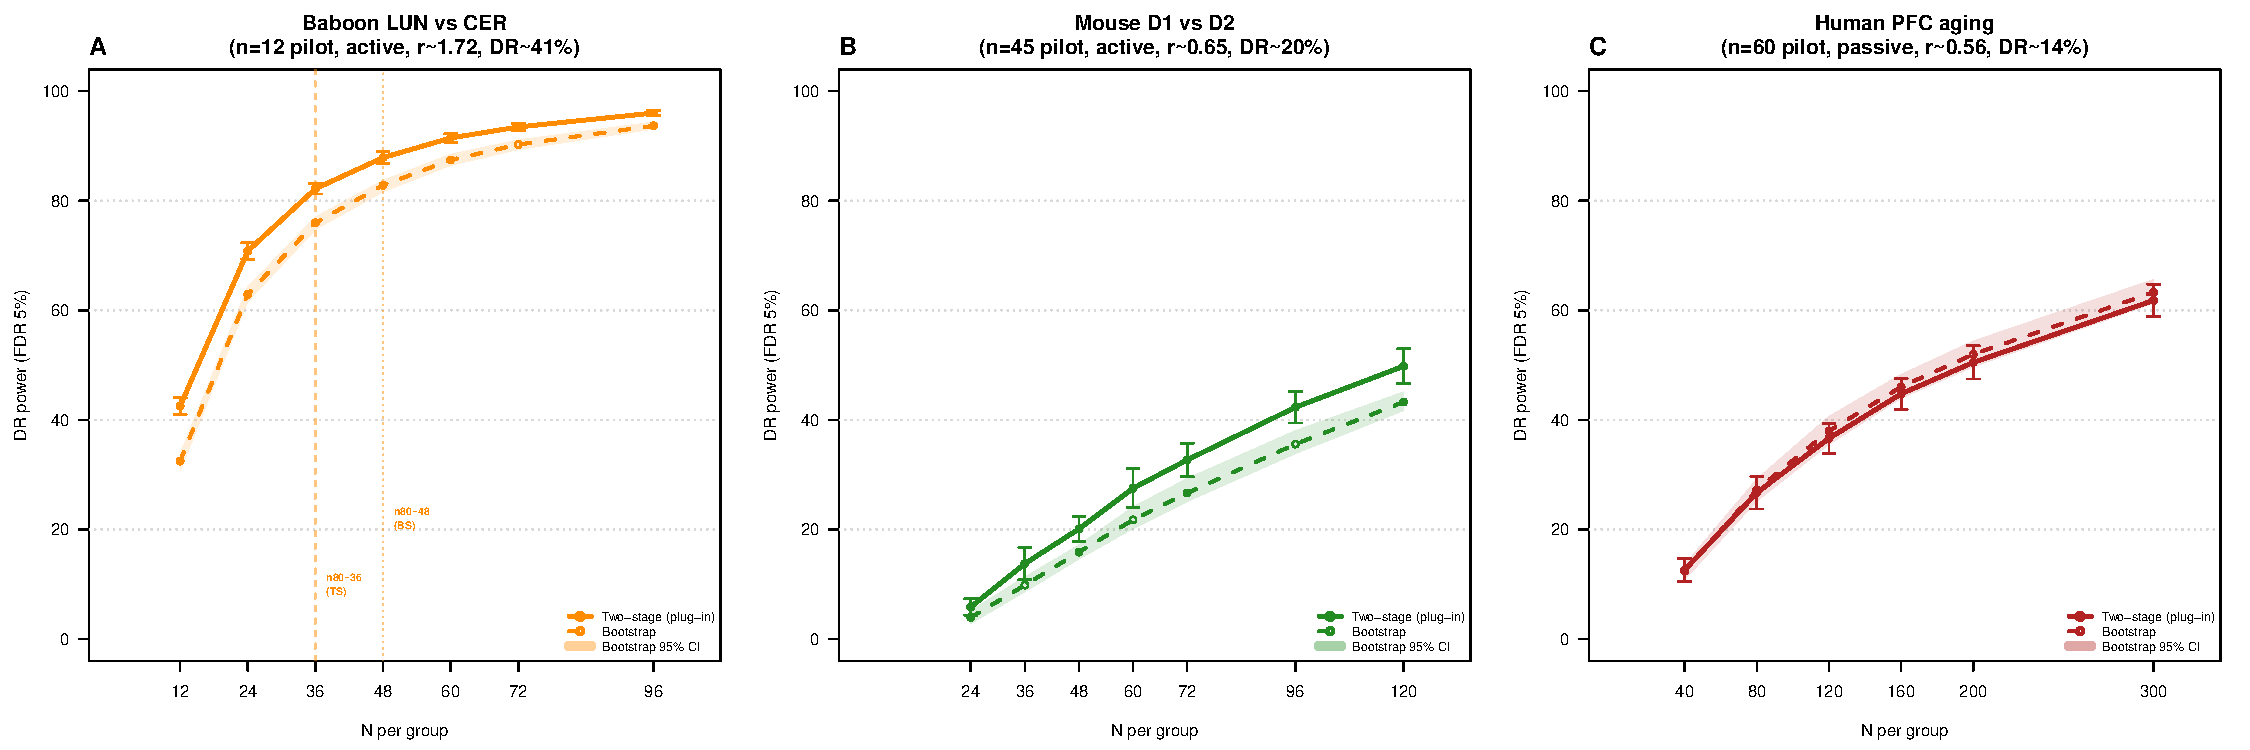
\includegraphics[width=\textwidth]{figures/bootstrap_summary.pdf}
\caption{Bootstrap vs.\ two-stage projected DR power across three pilot datasets.
Left: Baboon LUN vs.\ CER ($n=12$, active $B=12$, $m=1$).
Centre: Mouse D1 vs.\ D2 ($n=45$, active $B=6$).
Right: Seney MDD vs.\ Control ACC ($n=60$, passive).
Solid lines: two-stage plug-in power. Dashed lines: bootstrap mean power.
Shaded bands: 95\% bootstrap CI (pointwise).}
\label{fig:bootstrap_baboon}
\end{figure}

\begin{figure}[H]
\centering
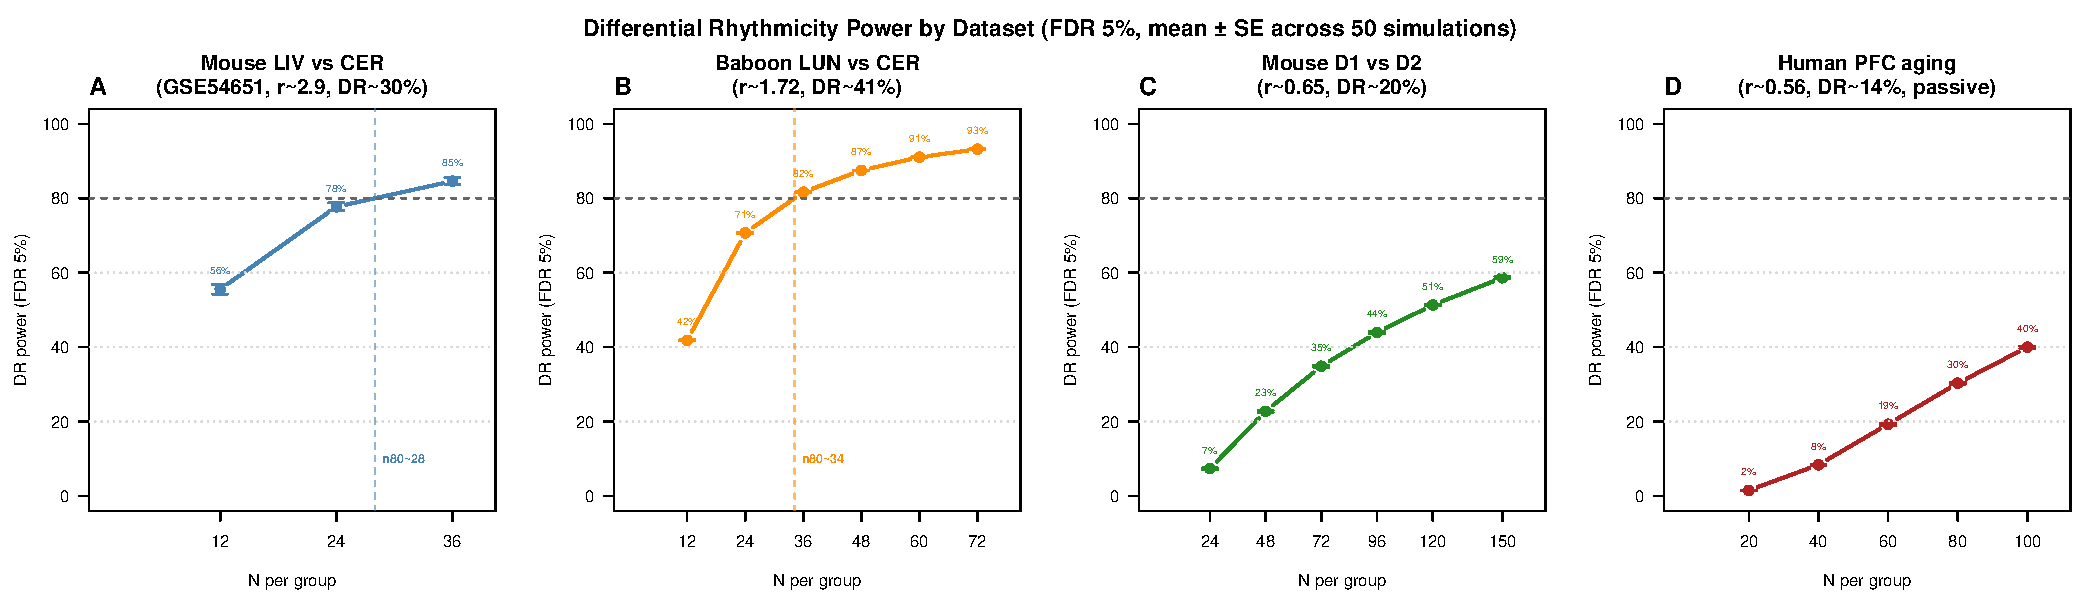
\includegraphics[width=\textwidth]{figures/multi_dataset_dr_power.pdf}
\caption{DR power vs.\ $N$ for four pilot datasets at FDR 5\%.}
\label{fig:multi_dr_power}
\end{figure}

\begin{figure}[H]
\centering

\includegraphics[width=\textwidth]{figures/bm_tradeoff.pdf}
\caption{B vs.\ m tradeoff across datasets.}
\label{fig:bm_tradeoff}
\end{figure}

\begin{figure}[H]
\centering
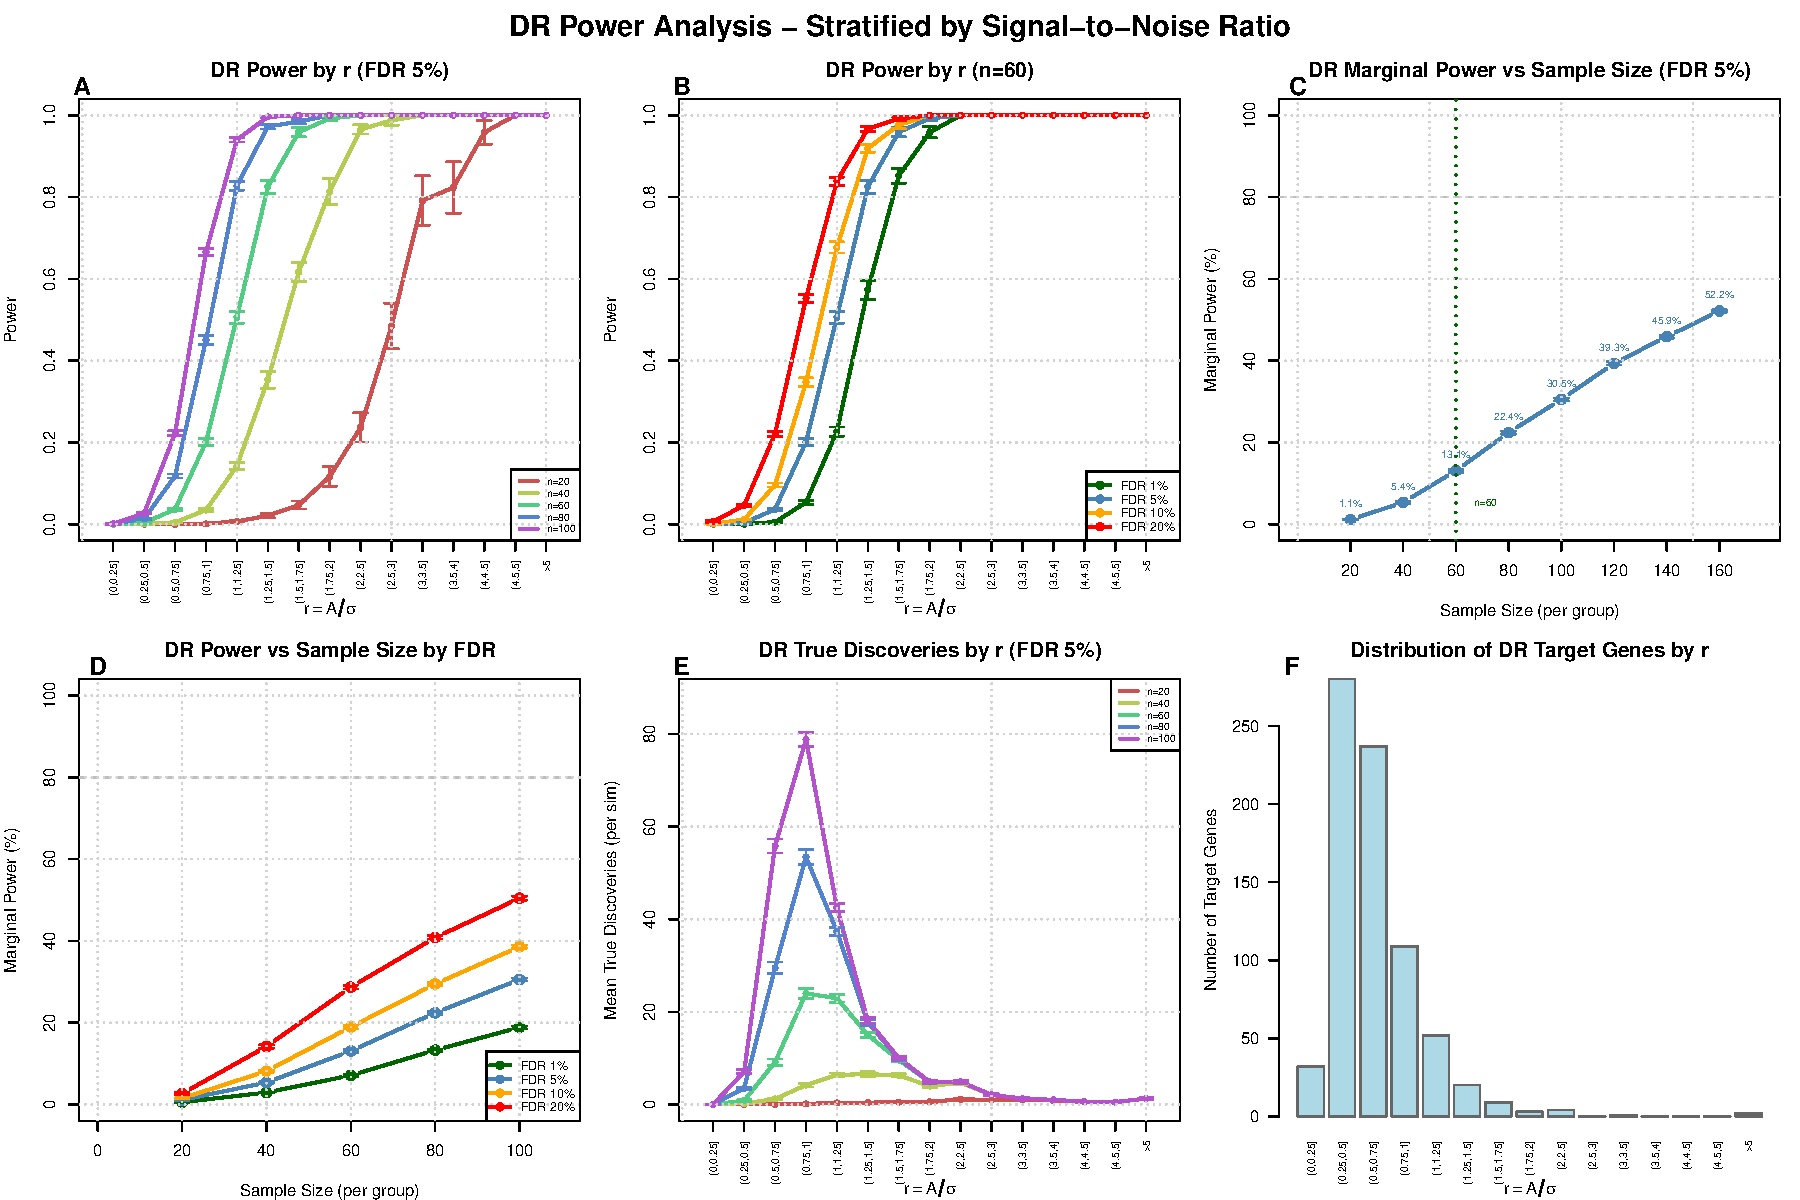
\includegraphics[width=\textwidth]{figures/dr_power.pdf}
\caption{DR power analysis. (A) Power by $r$ stratum at FDR 5\%. (B) Power by FDR threshold. (C) Marginal power vs.\ sample size. (D) Marginal power by FDR threshold. (E) True discoveries by $r$ stratum. (F) Empirical distribution of DR targets across $r$ strata.}
\label{fig:dr_power}
\end{figure}

\begin{figure}[H]
\centering
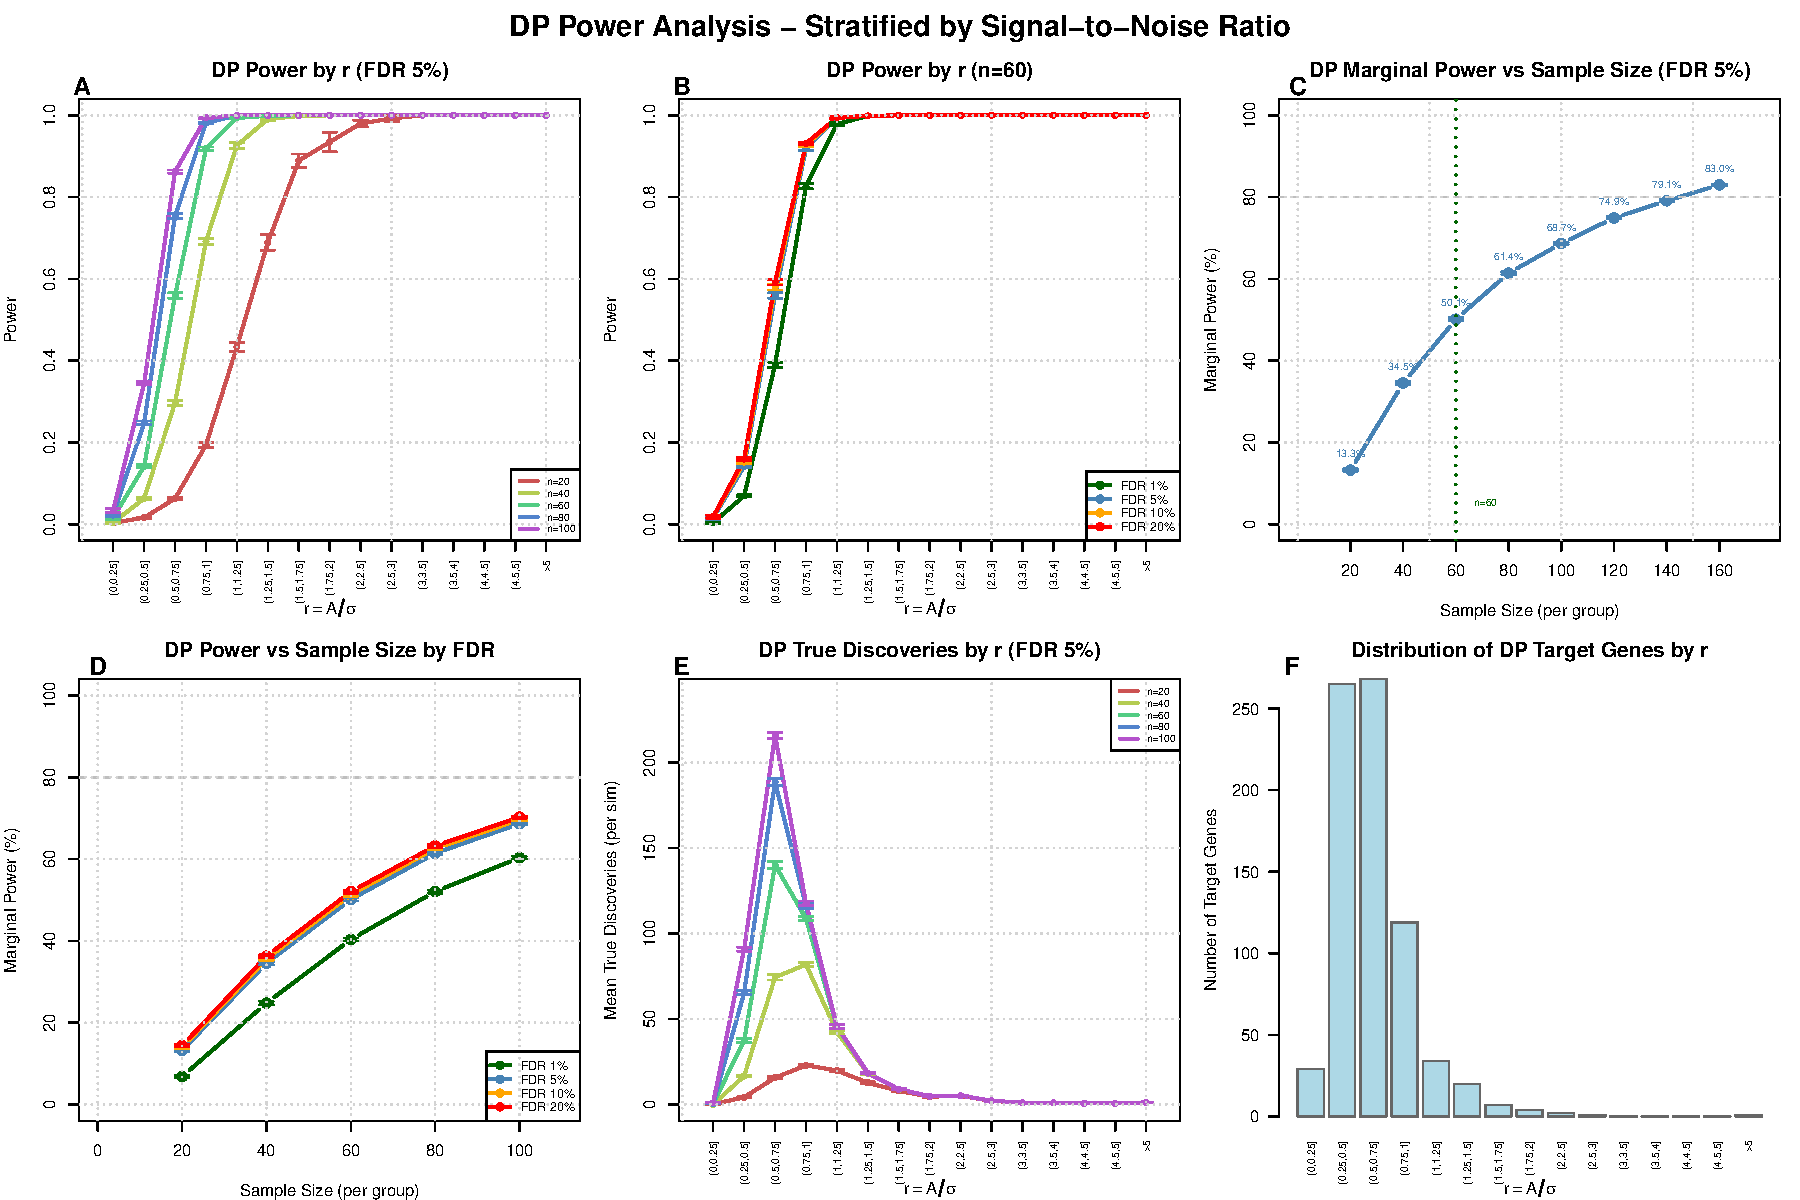
\includegraphics[width=\textwidth]{figures/dp_power.pdf}
\caption{DP power analysis ($\pm$6\,h phase shift).}
\label{fig:dp_power}
\end{figure}

\begin{figure}[H]
\centering
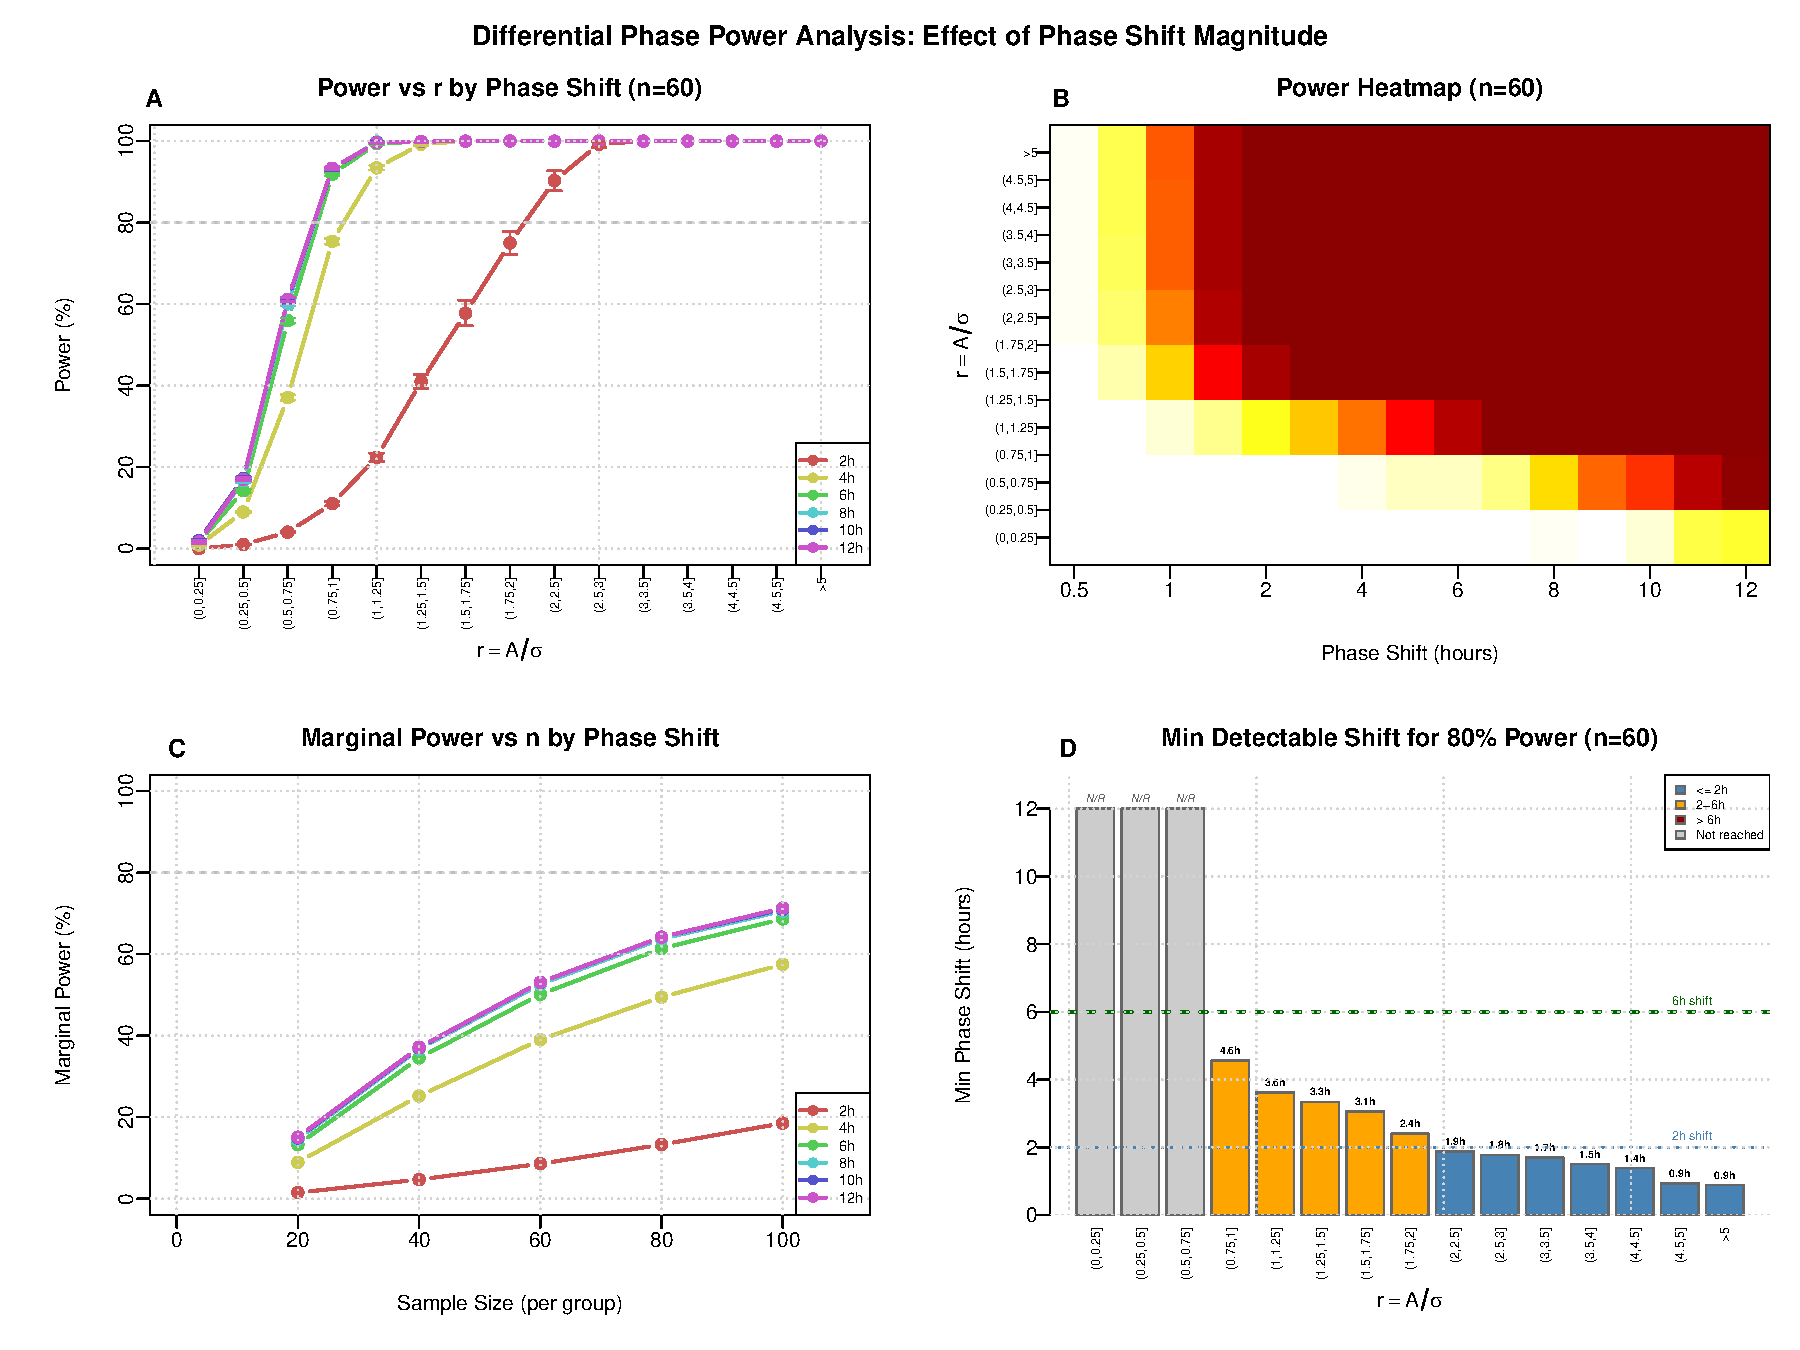
\includegraphics[width=\textwidth]{figures/phase_shift_abdf.pdf}
\caption{Phase shift sensitivity (5,000 genes, 50 simulations).}
\label{fig:phase_shift_abdf}
\end{figure}

\begin{figure}[H]
\centering
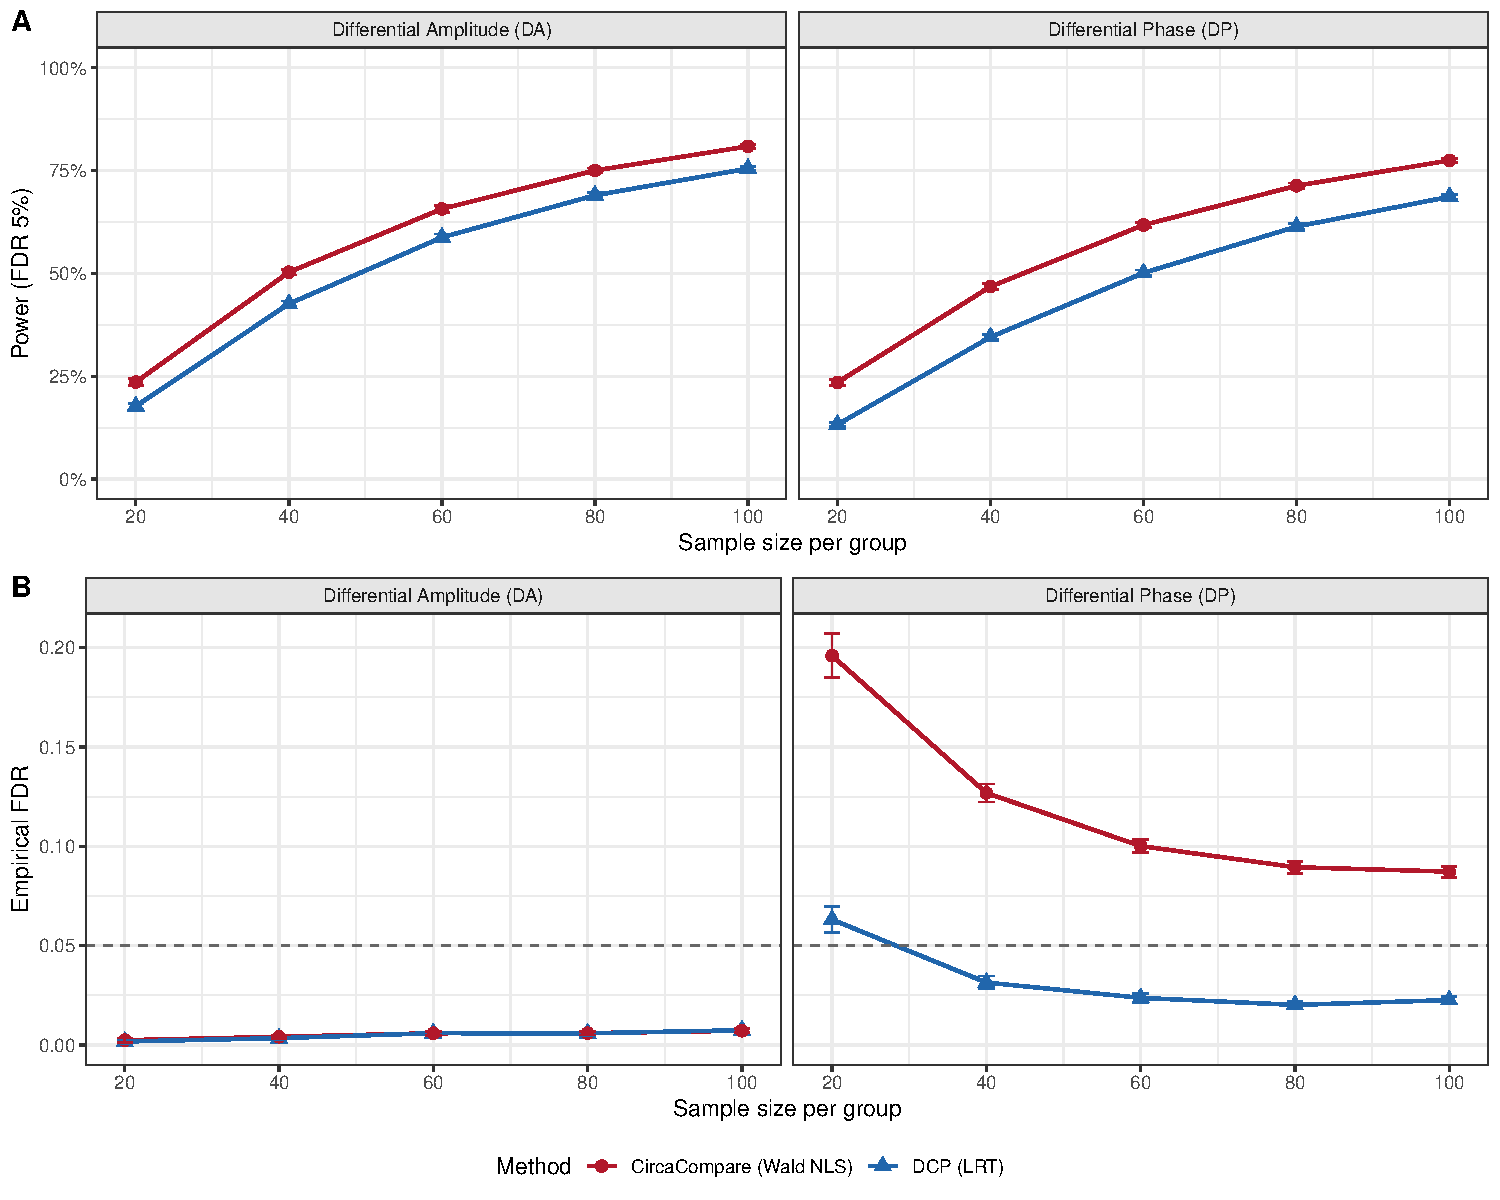
\includegraphics[width=\textwidth]{method_comparison/figures/method_comparison_combined.pdf}
\caption{Method comparison: DCP (LRT) vs.\ CircaCompare (Wald NLS) for DP.}
\label{fig:method_comparison}
\end{figure}
